%% FEUP THESIS STYLE for LaTeX2e
%% how to use feupteses (portuguese version)
%%
%% FEUP, JCL & JCF, 31 Jul 2012
%%
%% PLEASE send improvements to jlopes at fe.up.pt and to jcf at fe.up.pt
%%

%%========================================
%% Commands: pdflatex tese
%%           bibtex tese
%%           makeindex tese (only if creating an index) 
%%           pdflatex tese
%% Alternative:
%%          latexmk -pdf tese.tex
%%========================================

\documentclass[11pt,a4paper,twoside,openright]{report}

%% For iso-8859-1 (latin1), comment next line and uncomment the second line
\usepackage[utf8]{inputenc}
%\usepackage[latin1]{inputenc}

%% Portuguese version

%% MIEIC options
\usepackage[portugues,mieic]{feupteses}
%\usepackage[portugues,mieic,juri]{feupteses}
%\usepackage[portugues,mieic,final]{feupteses}
%\usepackage[portugues,mieic,final,onpaper]{feupteses}

%% Options: 
%% - portugues: titles, etc in portuguese
%% - onpaper: links are not shown (for paper versions)
%% - backrefs: include back references from bibliography to citation place

%% Uncomment the next lines if side by side graphics used
%\usepackage[lofdepth,lotdepth]{subfig}
%\usepackage{graphicx}
%\usepackage{float}

%% Include color package
\usepackage{color}
\definecolor{cloudwhite}{cmyk}{0,0,0,0.025}

%% Include source-code listings package
\usepackage{listings}
\lstset{ %
 language=C,                        % choose the language of the code
 basicstyle=\footnotesize\ttfamily,
 keywordstyle=\bfseries,
 numbers=left,                      % where to put the line-numbers
 numberstyle=\scriptsize\texttt,    % the size of the fonts that are used for the line-numbers
 stepnumber=1,                      % the step between two line-numbers. If it's 1 each line will be numbered
 numbersep=8pt,                     % how far the line-numbers are from the code
 frame=tb,
 float=htb,
 aboveskip=8mm,
 belowskip=4mm,
 backgroundcolor=\color{cloudwhite},
 showspaces=false,                  % show spaces adding particular underscores
 showstringspaces=false,            % underline spaces within strings
 showtabs=false,                    % show tabs within strings adding particular underscores
 tabsize=2,	                    % sets default tabsize to 2 spaces
 captionpos=b,                      % sets the caption-position to bottom
 breaklines=true,                   % sets automatic line breaking
 breakatwhitespace=false,           % sets if automatic breaks should only happen at whitespace
 escapeinside={\%*}{*)},            % if you want to add a comment within your code
 morekeywords={*,var,template,new}  % if you want to add more keywords to the set
}

\usepackage{pgfgantt}

%% Uncomment next line to set the depth of sectional units listed in the toc
%\setcounter{tocdepth}{3}

%% Uncomment to create an index (at the end of the document)
%\makeindex

%% Path to the figures directory
%% TIP: use folder ``figures'' to keep all your figures
\graphicspath{{figures/}}

%%----------------------------------------
%% TIP: if you want to define more macros, use an external file to keep them
%some macro definitions

% format
\newcommand{\class}[1]{{\normalfont\slshape #1\/}}

% entities
\newcommand{\Feup}{Faculdade de Engenharia da Universidade do Porto}

\newcommand{\svg}{\class{SVG}}
\newcommand{\scada}{\class{SCADA}}
\newcommand{\scadadms}{\class{SCADA/DMS}}

%%----------------------------------------

%%========================================
%% Start of document
%%========================================
\begin{document}

%%----------------------------------------
%% Information about the work
%%----------------------------------------
\title{Interference Aware Scheduling for Cloud Computing}
\author{Diogo Trindade Basto}

%% Uncomment next line for date of submission
%\thesisdate{11 de Fevereiro de 2014}

%% Uncomment next line for copyright text if used
%\copyrightnotice{Nome do Autor, 2008}

\supervisor{Orientador}{Jorge Manuel Gomes Barbosa}

%% Uncomment next line if necessary
%\supervisor{Co-orientador}{Nome de Outro Orientador}

%% Uncomment committee stuff in the final version
%\committeetext{Aprovado em provas públicas pelo Júri:}
%\committeemember{Presidente}{Nome do presidente do júri}
%\committeemember{Arguente}{Nome do arguente do júri}
%\committeemember{Vogal}{Nome do vogal do júri}
%\signature

%% Specify cover logo (in folder ``figures'')
\logo{uporto-feup.pdf}

%% Uncomment next line for additional text below the author's name (front page)
%\additionalfronttext{Preparação da Dissertação}

%%----------------------------------------
%% Preliminary materials
%%----------------------------------------

% remove unnecessary \include{} commands
\begin{Prolog}
  \chapter*{Resumo}

O Resumo fornece ao leitor um sumário do conteúdo da dissertação.
Deverá ser breve mas conter detalhe suficiente e, uma vez que é a porta
de entrada para a dissertação, deverá dar ao leitor uma boa impressão
inicial.

Este texto inicial da dissertação é escrito no fim e resume numa
página, sem referências externas, o tema e o contexto do trabalho, a
motivação e os objectivos, as metodologias e técnicas empregues, os
principais resultados alcançados e as conclusões.

Este documento ilustra o formato a usar em dissertações na \Feup.
São dados exemplos de margens, cabeçalhos, títulos, paginação, estilos
de índices, etc. 
São ainda dados exemplos de formatação de citações, figuras e tabelas,
equações, referências cruzadas, lista de referências e índices.
%Este documento não pretende exemplificar conteúdos a usar. 
É usado texto descartável, \emph{Loren Ipsum}, para preencher a
dissertação por forma a ilustrar os formatos.

Seguem-se umas notas breves mas muito importantes sobre a versão 
provisória e a versão final do documento. 
A versão provisória, depois de verificada pelo orientador e de 
corrigida em contexto pelo autor, deve ser publicada na página 
pessoal de cada estudante/dissertação, juntamente com os dois 
resumos, em português e em inglês; deve manter a marca da água, 
assim como a numeração de linhas conforme aqui se demonstra.

A versão definitiva, a produzir somente após a defesa, em versão 
impressa (dois exemplares com capas próprias FEUP) e em versão 
eletrónica (6 CDs com "rodela" própria FEUP), deve ser limpa da marca de 
água e da numeração de linhas e deve conter a identificação, na primeira 
página, dos elementos do júri respetivo. 
Deve ainda, se for o caso, ser corrigida de acordo com as instruções 
recebidas dos elementos júri.

Lorem ipsum dolor sit amet, consectetuer adipiscing elit. Sed vehicula
lorem commodo dui. Fusce mollis feugiat elit. Cum sociis natoque
penatibus et magnis dis parturient montes, nascetur ridiculus
mus. Donec eu quam. Aenean consectetuer odio quis nisi. Fusce molestie
metus sed neque. Praesent nulla. Donec quis urna. Pellentesque
hendrerit vulputate nunc. Donec id eros et leo ullamcorper
placerat. Curabitur aliquam tellus et diam. 

Ut tortor. Morbi eget elit. Maecenas nec risus. Sed ultricies. Sed
scelerisque libero faucibus sem. Nullam molestie leo quis
tellus. Donec ipsum. Nulla lobortis purus pharetra turpis. Nulla
laoreet, arcu nec hendrerit vulputate, tortor elit eleifend turpis, et
aliquam leo metus in dolor. Praesent sed nulla. Mauris ac augue. Cras
ac orci. Etiam sed urna eget nulla sodales venenatis. Donec faucibus
ante eget dui. Nam magna. Suspendisse sollicitudin est et mi. 

Phasellus ullamcorper justo id risus. Nunc in leo. Mauris auctor
lectus vitae est lacinia egestas. Nulla faucibus erat sit amet lectus
varius semper. Praesent ultrices vehicula orci. Nam at metus. Aenean
eget lorem nec purus feugiat molestie. Phasellus fringilla nulla ac
risus. Aliquam elementum aliquam velit. Aenean nunc odio, lobortis id,
dictum et, rutrum ac, ipsum. 

Ut tortor. Morbi eget elit. Maecenas nec risus. Sed ultricies. Sed
scelerisque libero faucibus sem. Nullam molestie leo quis
tellus. Donec ipsum. 

\chapter*{Abstract}

Here goes the abstract written in English.

Lorem ipsum dolor sit amet, consectetuer adipiscing elit. Sed vehicula
lorem commodo dui. Fusce mollis feugiat elit. Cum sociis natoque
penatibus et magnis dis parturient montes, nascetur ridiculus
mus. Donec eu quam. Aenean consectetuer odio quis nisi. Fusce molestie
metus sed neque. Praesent nulla. Donec quis urna. Pellentesque
hendrerit vulputate nunc. Donec id eros et leo ullamcorper
placerat. Curabitur aliquam tellus et diam. 

Ut tortor. Morbi eget elit. Maecenas nec risus. Sed ultricies. Sed
scelerisque libero faucibus sem. Nullam molestie leo quis
tellus. Donec ipsum. Nulla lobortis purus pharetra turpis. Nulla
laoreet, arcu nec hendrerit vulputate, tortor elit eleifend turpis, et
aliquam leo metus in dolor. Praesent sed nulla. Mauris ac augue. Cras
ac orci. Etiam sed urna eget nulla sodales venenatis. Donec faucibus
ante eget dui. Nam magna. Suspendisse sollicitudin est et mi. 

Fusce sed ipsum vel velit imperdiet dictum. Sed nisi purus, dapibus
ut, iaculis ac, placerat id, purus. Integer aliquet elementum
libero. Phasellus facilisis leo eget elit. Nullam nisi magna, ornare
at, aliquet et, porta id, odio. Sed volutpat tellus consectetuer
ligula. Phasellus turpis augue, malesuada et, placerat fringilla,
ornare nec, eros. Class aptent taciti sociosqu ad litora torquent per
conubia nostra, per inceptos himenaeos. Vivamus ornare quam nec sem
mattis vulputate. Nullam porta, diam nec porta mollis, orci leo
condimentum sapien, quis venenatis mi dolor a metus. Nullam
mollis. Aenean metus massa, pellentesque sit amet, sagittis eget,
tincidunt in, arcu. Vestibulum porta laoreet tortor. Nullam mollis
elit nec justo. In nulla ligula, pellentesque sit amet, consequat sed,
faucibus id, velit. Fusce purus. Quisque sagittis urna at quam. Ut eu
lacus. Maecenas tortor nibh, ultricies nec, vestibulum varius, egestas
id, sapien. 

Phasellus ullamcorper justo id risus. Nunc in leo. Mauris auctor
lectus vitae est lacinia egestas. Nulla faucibus erat sit amet lectus
varius semper. Praesent ultrices vehicula orci. Nam at metus. Aenean
eget lorem nec purus feugiat molestie. Phasellus fringilla nulla ac
risus. Aliquam elementum aliquam velit. Aenean nunc odio, lobortis id,
dictum et, rutrum ac, ipsum. 

Ut tortor. Morbi eget elit. Maecenas nec risus. Sed ultricies. Sed
scelerisque libero faucibus sem. Nullam molestie leo quis
tellus. Donec ipsum. Nulla lobortis purus pharetra turpis. Nulla
laoreet, arcu nec hendrerit vulputate, tortor elit eleifend turpis, et
aliquam leo metus in dolor. Praesent sed nulla. Mauris ac augue. Cras
ac orci. Etiam sed urna eget nulla sodales venenatis. Donec faucibus
ante eget dui. Nam magna. Suspendisse sollicitudin est et mi. 

Phasellus ullamcorper justo id risus. Nunc in leo. Mauris auctor
lectus vitae est lacinia egestas. Nulla faucibus erat sit amet lectus
varius semper. Praesent ultrices vehicula orci. Nam at metus. Aenean
eget lorem nec purus feugiat molestie. Phasellus fringilla nulla ac
risus. Aliquam elementum aliquam velit. Aenean nunc odio, lobortis id,
dictum et, rutrum ac, ipsum. 

Ut tortor. Morbi eget elit. Maecenas nec risus. Sed ultricies. Sed
scelerisque libero faucibus sem. Nullam molestie leo quis
tellus. Donec ipsum. 
 % the abstract
% \chapter*{Agradecimentos}
%\addcontentsline{toc}{chapter}{Agradecimentos}

Aliquam id dui. Nulla facilisi. Nullam ligula nunc, viverra a, iaculis
at, faucibus quis, sapien. Cum sociis natoque penatibus et magnis dis
parturient montes, nascetur ridiculus mus. Curabitur magna ligula,
ornare luctus, aliquam non, aliquet at, tortor. Donec iaculis nulla
sed eros. Sed felis. Nam lobortis libero. Pellentesque
odio. Suspendisse potenti. Morbi imperdiet rhoncus magna. Morbi
vestibulum interdum turpis. Pellentesque varius. Morbi nulla urna,
euismod in, molestie ac, placerat in, orci. 

Ut convallis. Suspendisse luctus pharetra sem. Sed sit amet mi in diam
luctus suscipit. Nulla facilisi. Integer commodo, turpis et semper
auctor, nisl ligula vestibulum erat, sed tempor lacus nibh at
turpis. Quisque vestibulum pulvinar justo. Class aptent taciti
sociosqu ad litora torquent per conubia nostra, per inceptos
himenaeos. Nam sed tellus vel tortor hendrerit pulvinar. Phasellus
eleifend, augue at mattis tincidunt, lorem lorem sodales arcu, id
volutpat risus est id neque. Phasellus egestas ante. Nam porttitor
justo sit amet urna. Suspendisse ligula nunc, mollis ac, elementum
non, venenatis ut, mauris. Mauris augue risus, tempus scelerisque,
rutrum quis, hendrerit at, nunc. Nulla posuere porta orci. Nulla dui. 

Fusce gravida placerat sem. Aenean ipsum diam, pharetra vitae, ornare
et, semper sit amet, nibh. Nam id tellus. Etiam ultrices. Praesent
gravida. Aliquam nec sapien. Morbi sagittis vulputate dolor. Donec
sapien lorem, laoreet egestas, pellentesque euismod, porta at,
sapien. Integer vitae lacus id dui convallis blandit. Mauris non
sem. Integer in velit eget lorem scelerisque vehicula. Etiam tincidunt
turpis ac nunc. Pellentesque a justo. Mauris faucibus quam id
eros. Cras pharetra. Fusce rutrum vulputate lorem. Cras pretium magna
in nisl. Integer ornare dui non pede. 

\vspace{10mm}
\flushleft{O Nome do Autor}
  % the acknowledgments
% \cleardoublepage
\thispagestyle{plain}

\vspace*{8cm}

\begin{flushright}
   \textsl{``You should be glad that bridge fell down. \\
           I was planning to build thirteen more to that same design''} \\
\vspace*{1.5cm}
           Isambard Kingdom Brunel
\end{flushright}
    % initial quotation if desired
  \cleardoublepage
  \pdfbookmark[0]{Conteúdo}{contents}
  \tableofcontents
  \cleardoublepage
  \pdfbookmark[0]{Lista de Figuras}{figures}
  \listoffigures
  \cleardoublepage
  \pdfbookmark[0]{Lista de Tabelas}{tables}
  \listoftables
  \chapter*{Abreviaturas e Símbolos}
%\addcontentsline{toc}{chapter}{Abbreviations}
\chaptermark{ABREVIATURAS E SÍMBOLOS}

\begin{flushleft}
\begin{tabular}{l p{0.8\linewidth}}
API      & Application Programming Interface\\
CERN & Conseil Européen pour la Recherche Nucléaire\\
%IaaS & Infrastructure as a Service\\
KVM & Kernel-based Virtual Machine\\
NSA & National Security Agency\\
%PaaS & Platform as a Service\\
QoS & Quality of Service\\
%SaaS & Software as a Service\\
SLA & Service Level Agreement\\
%VM & Virtual Machine\\
\end{tabular}
\end{flushleft}

  % the list of abbreviations used
\end{Prolog}

%%----------------------------------------
%% Body
%%----------------------------------------

\StartBody

%% TIP: use a separate file for each chapter
\chapter{Introdução} \label{chap:intro}

\section*{}

Nuvens computacionais são um serviço emergente na indústria tecnológica, pois permitem computação a um custo reduzido. A própria tecnologia é apenas a adaptação de outras tecnologias existentes para responder a um crescimento de utilização de serviços na \textit{internet}. Este serviço disponibilizado ao público por empresas como a Google, Amazon ou Microsoft permite a expansão do poder computacional aos utilizadores conforme as suas necessidades, eliminando um investimento inicial e possibilitando o crescimento do serviço. Grandes organizações, como o caso do CERN e NSA, utilizam redes computacionais internas para disponibilizar o poder computacional que as suas tarefas diárias necessitam, não limitando cada colaborador ao poder do seu computador pessoal, permitindo a aproveitação dos recursos organizacionais para a conclusão de tarefas mais rapidamente. 

A presente dissertação apresentará um método para melhorar o serviço das nuvens computacionais através dum escalonamento de tarefas mais consciente sobre o processo de virtualização e das interferências que o mesmo provoca na realização de tarefas nos nós computacionais.

% O primeiro capítulo da dissertação deve servir para apresentar o
% enquadramento e a moti\-va\-ção do trabalho e para identificar e
% definir os problemas que a dissertação aborda.
% Deve resumir as metodologias utilizadas no trabalho e termina
% apresentando um breve resumo de cada um dos capítulos
% posteriores.

% Este documento ilustra o formato a usar em dissertações na \Feup, não
% servindo de exemplo sobre os conteúdos a usar.
% São dados exemplos de margens, cabeçalhos, títulos, paginação, estilos
% de índices, etc. 
% São ainda dados exemplos de formatação de citações, figuras e tabelas,
% equações, referências cruzadas, lista de referências e índices.

% Uma recolha de normas existentes sobre este assunto pode ser
% encontrada em~\cite{kn:Mat93}. 

% \begin{quote}
%   ``Like the Abstract, the Introduction should be written to engage the
%   interest of the reader. It should also give the reader an idea of
%   how the dissertation is structured, and in doing so, define the
%   thread of the contents.''~\cite[chap.\ Introduction]{kn:Tha01} 
% \end{quote}

% Neste primeiro capítulo ilustra-se a utilização de citações e de
% referências biblio\-grá\-fi\-cas.
% Para além de dar um exemplo de utilização de uma citação, a citação
% anterior, introduz uma referência que pode ser consultada, entre
% muitas outras referências bibliográficas
% interessantes~\cite{kn:Tha01,kn:PP05}. 

% \section{Contexto} \label{sec:context}

% Esta secção descreve a área em que o trabalho se insere, podendo
% referir um eventual projeto de que faz parte e apresentar uma breve
% descrição da empresa onde o trabalho decorreu.

% Lorem ipsum~\cite{kn:Lip08} dolor sit amet, consectetuer adipiscing
% elit. 


\section{Motivação e Objetivos} \label{sec:goals}

A otimização da utilização dos recursos disponíveis permite melhorias na qualidade do serviço (QoS) fornecido aos utilizadores, através de serviços mais rápidos e responsivos, e menor gastos por parte dos fornecedores, através de reduções energéticas devido a menores períodos de utilização e cumprimento dos acordos da qualidade do serviço (SLA), influenciando positivamente todas as partes interessadas. É, portanto, uma área de interesse estudar otimizações possíveis que contribuam para a eficiência do serviço. Uma parte principal do funcionamento de uma nuvem é o escalonador, responsável por atribuir as tarefas aos nós disponíveis. Esta atribuição é feita em linha, aquando da chegada de uma tarefa, o escalonador deverá avaliar os vários nós da rede computacional e despachar a tarefa para o nó que possua a melhor avaliação.
Esta avaliação tem em conta as características de uma tarefa, através da especificação do pedido ou por execução da mesma temporariamente e medir os recursos exigidos, e as capacidades e quantidade de trabalho de cada nó. Técnicas de escalonamento atuais não tem em conta a interação entre tarefas, um dos principais culpados nos atrasos na nuvem, devido às tecnologias de virtualização e arquitetura do \textit{hardware} usados. Quando duas tarefas com utilizações de recursos semelhantes, por exemplo ambas tem bastante acesso a disco para recolha e escrita de dados com pouco tratamento dos mesmos a nível do processador, são atribuídas ao mesmo nó, que terá espaço de disco para ambas, as máquinas virtuais irão interferir entre si no acesso a recursos que não podem ser divididos para cada virtualização devido à sua arquitetura, neste caso, o barramento de dados. 

Esta dissertação tem como objetivo desenvolver um escalonador que utilize métricas de interferência para poder reduzir o impacto das mesmas na nuvem. Para isso será estudada a interferência entre vários tipos de tarefas, em bibliografia existente, e utilizado um simulador de uma nuvem computacional para avaliar o desempenho do escalonador. Para efeitos de avaliação de resultados será utilizado um escalonador de código aberto, utilizado atualmente na indústria, o \textit{Filter Scheduler} do OpenStack \cite{gong2012nova}. Para simulação será utilizado o SimGrid e a arquitetura de rede será idêntica à utilizada no CERN, podendo para simulação de tarefas ser utilizado os dados de utilização da sua nuvem ou criadas novas tarefas de uso científico geral, como especificadas em \cite{mehta2013pegasus}.



% Apresenta a motivação e enumera os objetivos do trabalho terminando
% com um resumo das metodologias para a prossecução dos objetivos.


\section{Estrutura da Dissertação} \label{sec:struct}

Os capítulos seguintes deste relatório encontram-se da forma seguinte. O capítulo 2 apresenta o estado da arte na área de computação em nuvem, sendo específico na área de escalonamento e de interferências na virtualização. O capítulo 3 apresenta os dados sobre interferência recolhidos e explica o impacto dos mesmos na rede computacional. O capítulo 4 descreve detalhes de implementação que serão utilizados para a realização do trabalho e os métodos utilizados para avaliação de resultados. O capítulo 5 apresentará as conclusões retiradas da preparação de dissertação e o plano de trabalho a seguir.

% Para além da introdução, esta dissertação contém mais x capítulos.
% No capítulo~\ref{chap:sota}, é descrito o estado da arte e são
% apresentados trabalhos relacionados. 
% %\todoline{Complete the document structure.}
% No capítulo~\ref{chap:chap3}, ipsum dolor sit amet, consectetuer
% adipiscing elit.
% No capítulo~\ref{chap:chap4} praesent sit amet sem. 
% No capítulo~\ref{chap:concl}  posuere, ante non tristique
% consectetuer, dui elit scelerisque augue, eu vehicula nibh nisi ac
% est. 
 
\chapter{Estado da Arte} \label{chap:sota}

\section*{}

O presente capítulo identificará referências bibliográficas sobre o presente estado da computação em nuvem, as suas utilizações e proliferação. De seguida, apresenta trabalhos anteriores sobre escalonamento de tarefas na nuvem, seguido de análise de trabalhos sobre interferências entre máquinas virtuais e sobre o simulador a utilizar, SimGrid. 

% Neste capítulo é descrito o estado da arte e são
% apresentados trabalhos relacionados para mostrar o que existe no
% mesmo domínio e quais os problemas em aberto.
% Deve deixar claro que existe uma oportunidade de desenvolvimento que
% cobre alguma falha concreta .

% O capítulo deve também efetuar uma revisão tecnológica às principais
% ferramentas utilizáveis no âmbito do projeto, justificando futuras
% escolhas.

\section{Computação em Nuvem}

No artigo \cite{armbrust2010view}, os autores apresentam sucintamente a utilidade dos serviços de computação oferecidos atualmente e os principais obstáculos e oportunidades de desenvolvimento. Em \cite{buyya2009cloud} os autores apresentam a nuvem como a futura quinta utilidade e o modelo de negócio que é utilizado pelos fornecedores de serviço ainda hoje. Para o cumprimento dos contratos estipulados e combater os atrasos são provisionados recursos a mais dos que foram contratados, diminuindo a eficiência da nuvem, como explicado em \cite{armbrust2010view, nathuji2010q ,corradi2012vm}. Em \cite{wen2012comparison} é feita a comparação entre os dois principais programas de gestão de nuvens, OpenStack e OpenNebula. Os autores de \cite{vecchiola2009high} demonstram a utilidade da computação em nuvem na comunidade científica, apresentando um estudo sobre a utilização do poder computacional na classificação de dados de expressão genética e compilação de imagens de ressonâncias magnéticas. Devido à disponibilização dos dados e configuração do CERN para a realização desta dissertação, foi escolhido o OpenStack por ser o mesmo utilizado pela organização \cite{openstackcern}. O algoritmo a ser replicado para efeitos de teste e avaliação de resultados está descrito em \cite{gong2012nova}.

% Neste capítulo é ilustrada a utilização de macros \LaTeX\ para definir
% entradas no índice remissivo e são feitas diversas referências
% bibliográficas, usando-se texto de um artigo apresentado na Conferência 
% XATA2006~\cite{kn:MVL06-xata}.

% Nos últimos tempos têm surgido diversas soluções, apresentadas por
% empresas do sector Automação de Sistemas para a disponibilização de
% sistemas \scadadms{} na \textit{Web}.

\section{Escalonamento de Tarefas em Nuvens de Computação}\label{sec:escalonamento}

Existe na área das nuvens de computação bastante bibliografia teórica e prática sobre escalonamento. Em \cite{abraham2000nature} é estudada a utilização de algoritmos probabilísticos, como algoritmos genéticos, arrefecimento simulado e pesquisa tabu. Em \cite{daoud2008high} é descrito um algoritmo de escalonamento por listagem. No entanto as duas soluções requerem um conhecimento à priori da totalidade das tarefas que vão ser executadas, o que não é possível na maioria dos casos. Em \cite{topcuoglu2002performance} os autores apresentam os algoritmos de primeiro tempo de chegada heterogéneo e caminho crítico no processador, algoritmos que são focados na rapidez da resposta. Vários trabalhos focam-se no escalonamento de tarefas de área científica, cuja topologia é conhecida e possa ser dividida entre várias sub-tarefas diferentes. Este escalonamento é NP-completo. Os autores de \cite{gupta2012optimizing} utilizam uma heurística que aproxima as sub-tarefas dentro da rede, de maneira a acelerar o processo de partilha de dados entre as tarefas e tenta que tarefas iguais fiquem em nós de igual capacidade, para que possam todos trabalhar à sua velocidade máxima. O trabalho em \cite{chen2009ant} segue a mesma lógica, utilizando um algoritmo de colónia de formigas. Os autores de \cite{su2013cost} utilizam ótimos de Pareto para determinar o melhor nó para alocar as tarefas, melhorando sucessivamente a sua solução. Em \cite{zheng2013budget} é demonstrada uma extensão ao algoritmo de escalonamento primeiro tempo de chegada heterogéneo. 

% \emph{Scalable Vector Graphics}\index{SVG}\index{XML!SVG} é uma
% linguagem em formato XML que descreve gráficos de duas dimensões. 
% Este formato padronizado pela W3C (\emph{World Wide Web Consortium})
% é livre de patentes ou direitos de autor e está totalmente
% documentado, à semelhança de outros W3CN
% standards~\cite{kn:svgdoc}.

% Sendo uma linguagem XML, o \svg{} herda uma série de vantagens: a
% possibilidade de transformar \svg{} usando técnicas como
% XSLT\index{XML!XSLT}, de embeber \svg{} em qualquer documento
% XML\index{XML} usando \textit{namespaces} ou até de  
% estilizar \svg{} recorrendo a CSS\index{CSS} (\emph{Cascade Style Sheets}). 
% De uma forma geral, pode dizer-se que \svg{}s interagem bem com as
% atuais tecnologias ligadas ao XML e à Web, tal como referido
% em~\cite{kn:svgibm,kn:svgw3c}.

%\subsection{Heurísticas de escalonamento}

\section{Tecnologias de Virtualização}
Virtualização é a tecnologia que permite a um único computador isolar as várias tarefas que são executadas simultaneamente, sendo controlados por um monitor de maquinas virtuais em cada nó, o hipervisor. Em \cite{gu2012state} são apresentadas os hipervisores mais utilizados no mercado, programas que criam automaticamente em cada computador as máquinas virtuais necessárias para a execução de tarefas, concluindo com a listagem de problemas comuns entre eles. São também comparados e testados vários hipervisores em \cite{younge2011analysis}, obtendo resultados que favorecem o KVM para nuvens de computação de alto rendimento. 
Em \cite{cucinotta2011providing} é sugerido um escalonamento de tarefas a nível de nós individuais, ficando cada nó responsável por garantir a qualidade do serviço, realocando recursos a cada máquina virtual conforme necessário.

\subsection{Interferências em Tecnologias de Virtualização}\label{sec:interferencia} 
A interferência entre máquinas virtuais no mesmo anfitrião começou por ser estudada em \cite{koh2007analysis}, apresentando motivos para os atrasos observados, executando testes experimentais para conjuntos de duas máquinas virtuais simultâneas e usando regressão linear para prever conjuntos não testados. O estudo de interferência em tarefas que requerem comunicações dentro da rede em \cite{pu2010understanding}, utilizando tarefas limitadas por poder de computacional ou velocidade da rede, demonstra o efeito que a concorrência em componentes partilhados provoca no atraso das tarefas e conclui que a combinação de tarefas com usos de componentes diferentes leva ao menor efeito de interferência. Os autores de \cite{nathuji2010q} determinam que para as qualidade de serviço ser obedecida, cada nó deverá ter um espaço livre para poder alocar mais espaço a uma das virtualizações, não sendo eficiente na utilização dos recursos a troco de oferecer um serviço mais fidedigno. Em \cite{zhu2012performance} são construídos modelos de interferência entre máquinas virtuais, utilizando o modelo e um conjunto de regras para determinar se duas tarefas podem ser consolidadas no mesmo nó. Outra metodologia de recolha de dados sobre a interferência é descrita em \cite{govindan2011cuanta}, estudando a degradação de tarefas e relacionar o mesmo com a utilização de memória \textit{cache}.



\section{SimGrid}\label{sec:simgrid} 
SimGrid é a plataforma de simulação a ser utilizada para teste do algoritmo desenvolvido. Os autores de \cite{casanova2001sg} e \cite{legrand2003sg} demonstram casos de uso do simulador para testar algoritmos de escalonamento em versões anteriores da plataforma, podendo-se encontrar em \cite{casanova2008sg} um estudo com a versão mais recente. 


\section{Conclusões}
O estudo da bibliografia revela a importância das nuvens computacionais para a indústria na atualidade. Sendo uma tecnologia ainda em desenvolvimento, apresenta vulnerabilidades já identificadas que podem ser corrigidas para melhorar o serviço atual. Os estudos sobre interferência mostram uma redução de desempenho para valores até um terço do original entre um par de tarefas, podendo-se concluir que as tarefas executadas em série em vez de paralelizadas levariam a um desempenho superior. Esta interferência devido a recursos partilhados, por exemplo memória \textit{cache}, impossíveis de serem divididos por um hipervisor pode ser combatida com a adaptação de \textit{hardware} que não utilize partilha de recursos ou a adaptação da atribuição de tarefas para verificar a consolidação de tarefas com pouca interferência. 

% \begin{ganttchart}{1}{16}
% 	\ganttitlelist{Novembro,Dezembro,Janeiro,Fevereiro}{4}\\
% 	\gantttitlelist{1,2,3,4,1,2,3,4,1,2,3,4,1,2,3,4}{1}\\
% 	\ganttbar{Estudo}{1}{2}\\
% 	%\gantttitlelist{Março,Abril,Maio,Junho}{4}\\
% 	%\gantttitlelist{1,2,3,4,1,2,3,4,1,2,3,4,1,2,3,4}{1}\\
% \end{ganttchart}

% No final do capítulo deverá ser apresentado um resumo com as 
% principais conclusões que se podem tirar. 

\chapter{Interferência entre Máquinas Virtuais}\label{chap:interferencia}

\section*{}


% Este capítulo deve começar por fazer uma apresentação detalhada do
% problema a resolver\footnote{Na introdução a apresentação do
%   problema foi breve.} podendo mesmo, caso se justifique,
% constituir-se um capítulo com essa finalidade.

% Deve depois dedicar-se à apresentação da solução sem detalhes de
% implementação. 
% Dependendo do trabalho, pode ser uma descrição mais teórica, mais
% ``arquitetural'', etc.

Os sistemas de virtualização são a principal tecnologia para o funcionamento das nuvens computacionais. Os hipervisores controlam a alocação de recursos a cada máquina virtual, no entanto existem recursos fisicamente partilhados, impossíveis de distribuir uniformemente, sendo a sua utilização ditada pelos controladores de \textit{hardware}. Não sendo possível aos hipervisores resolver esta alocação, cada VM alocada pode-se apoderar da totalidade dos recursos partilhados e impedir as restantes de executarem o seu trabalho. O trabalho desta dissertação pretende minimizar estas ocorrências, através do estudo das interferências e executar uma alocação de tarefas a cada nó consciente do impacto das mesmas no rendimento das tarefas que já se encontram em execução ou em espera nesse nó.

\section{Dados de Interferência}

Na Figura \ref{fig:modeloshell} é possível visualizar o rendimento de execução de dois comandos de \textit{shell} em máquinas virtuais separadas\footnote{As máquinas virtuais possuem recursos iguais e o hospedeiro possui capacidade igual ou superior à soma das duas.}. O resultado é normalizado ao tempo de execução do comando \textbf{grep} e os restantes valores são obtidos através das fórmulas . O desempenho da tarefa \textbf{grep} em conjunto com a \textbf{povray} tem um rendimento perto de perfeito, quase atingindo o valor 2. No entanto todas as outras combinações degradam o desempenho, atingindo um mínimo quando dois \textbf{grep} são executados paralelamente. 

\begin{figure}[t]
  \begin{center}
    \leavevmode
    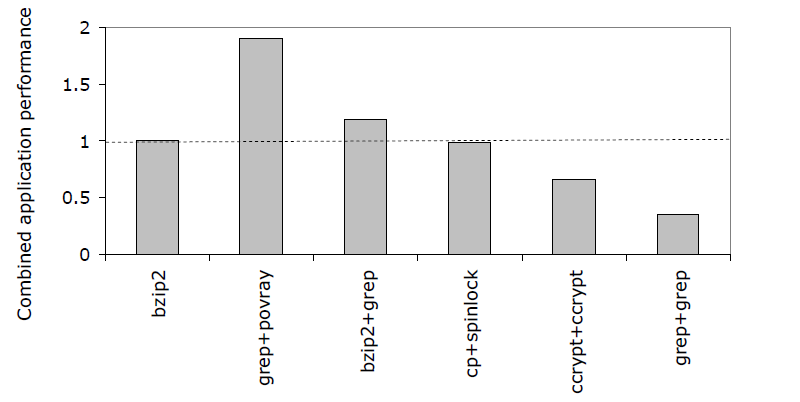
\includegraphics[width=0.86\textwidth]{interferenciashell.png}
    \caption{Tempo de execução normalizado de duas máquinas virtuais a executar commandos da \textit{shell}. Fonte: \cite{koh2007analysis}}
    \label{fig:modeloshell}
  \end{center}
\end{figure}

\section{Abordagem}



% Neste capítulo apresentam-se exemplos de formatação de figuras e
% tabelas, equações e referências cruzadas.

% Apresenta-se de seguida um exemplo de equação, completamente fora do contexto:
% \begin{eqnarray}
% CIF_1: \hspace*{5mm}F_0^j(a) &=& \frac{1}{2\pi \iota} \oint_{\gamma} \frac{F_0^j(z)}{z - a} dz\\
% CIF_2: \hspace*{5mm}F_1^j(a) &=& \frac{1}{2\pi \iota} \oint_{\gamma} \frac{F_0^j(x)}{x - a} dx \label{eq:cif}
% \end{eqnarray}

% Na Equação~\ref{eq:cif} lorem ipsum dolor 

% A arquitetura do visualizador assenta sobre os seguintes conceitos
% base~\cite{kn:ZPMD97}: 

% \begin{itemize}
% \item \textbf{Componentes} --- Suspendisse auctor mattis augue \emph{push};
% \item \textbf{Praesent} --- Sit amet sem maecenas eleifend facilisis leo;
% \item \textbf{Pellentesque} --- Habitant morbi tristique senectus et netus.
% \end{itemize}


% É apresentado na Figura~\ref{fig:arch} %da página~\pageref{fig:arch}
% um exemplo de figura flutuante.

% \begin{figure}[t]
%   \begin{center}
%     \leavevmode
%     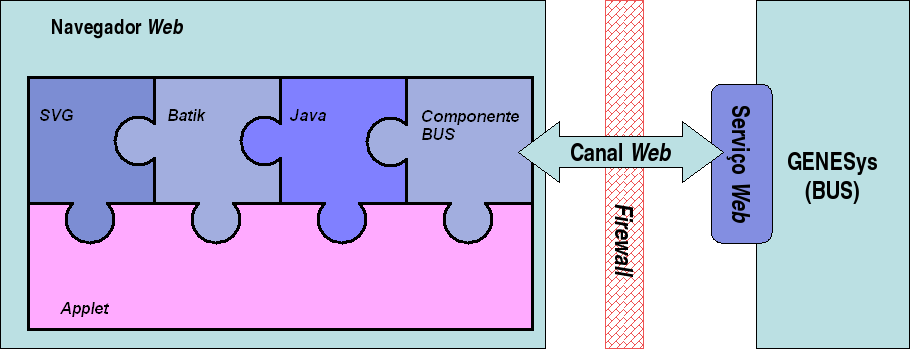
\includegraphics[width=0.86\textwidth]{puzzle}
%     \caption{Arquitectura da Solução Proposta}
%     \label{fig:arch}
%   \end{center}
% \end{figure}


% É apresentado na Tabela~\ref{tab:exemplo1} um exemplo de tabela
% flutuante e na Tabela~\ref{tab:exemplo2} um exemplo de tabela
% flutuante, um pouco mais complicada.

% \begin{table}[t]
%   \centering
%   \caption{Uma Tabela Simples}
% \begin{tabular}{| l | p{45mm} |}
% 	\hline
% \textbf{Acrónimo} & \textbf{Significado}\\
% 	\hline
% 	\hline
%         ADT   & \emph{Abstract Data Type}\\\hline
%         ANDF  & \emph{Architecture-Neutral Distribution Format}\\\hline
%         API   & \emph{Application Programming Interface}\\
% 	\hline
% \end{tabular}
%   \label{tab:exemplo1}
% \end{table}



% \begin{table}[t]
%   \centering
%   \caption{Uma Tabela Mais Complicada}
% \begin{tabular}{|c|r@{.}lr@{.}lr@{.}l||r|}
% 	\hline
% \multicolumn{8}{|c|}
% 	{\rule[-3mm]{0mm}{8mm}Iteração $k$ de $f(x_n)$} \\
% \textbf{\em k}
% 	& \multicolumn{2}{c}{$x_1^k$}
% 	& \multicolumn{2}{c}{$x_2^k$}
% 	& \multicolumn{2}{c||}{$x_3^k$}
% 	& comentários \\ \hline \hline
% 0   & -0&3                 & 0&6                 &  0&7   & - \\
% 1   &  0&47102965 & 0&04883157 & -0&53345964  & $\delta<\epsilon$ \\
% 2   &  0&49988691 & 0&00228830 & -0&52246185  & $\delta < \varepsilon$ \\
% 3   &  0&49999976 & 0&00005380 & -0&523656   &   $N$ \\
% 4   &  0&5                 & 0&00000307 & -0&52359743  & \\
% \vdots	& \multicolumn{2}{c}{\vdots}
% 	& \multicolumn{2}{c}{$\ddots$}
% 	& \multicolumn{2}{c||}{\vdots}  & \\
% 7   &  0&5   & 0&0    & \textbf{-0}&\textbf{52359878}
% 		 & $\delta<10^{-8}$ \\ \hline
% \end{tabular}
%   \label{tab:exemplo2}
% \end{table}



\section{Resumo e Conclusões}



%\chapter{Implementação}\label{chap:implementacao}

\section*{}

Este capítulo pode ser dedicado à apresentação de detalhes de nível
mais baixo relacionados com o enquadramento e implementação das
soluções preconizadas no capítulo anterior.
Note-se no entanto que detalhes desnecessários à compreensão do
trabalho devem ser remetidos para anexos.

Dependendo do volume, a avaliação do trabalho pode ser incluída neste
capítulo ou pode constituir um capítulo separado.

\section{Secção Exemplo}

%\todofigure{Inserir uma figura sobre o Map/Reduce}

Lorem ipsum dolor sit amet, consectetuer adipiscing elit. Integer
hendrerit commodo ante. Pellentesque nibh libero, aliquam at, faucibus
id, commodo a, velit. 
%\todoline{Escrever sobre o map/reduce}
Duis eleifend sem eget leo. Morbi in est. Suspendisse magna sem,
varius nec, hendrerit non, tincidunt quis, quam. Aenean congue. 
%\todolines{A short entry in the list of todos}{A very long todonote
%  that certainly will fill more than a single line in the list of
%  todos. Just to make sure let's add some more text.} 
Vivamus vel est sit amet sem iaculis posuere. Cras mollis, enim vel
gravida aliquam, libero nunc ullamcorper dui, ullamcorper sodales
lectus nulla sed urna. Morbi aliquet porta risus. 
Proin vestibulum ligula a purus. Maecenas a nulla. 
Maecenas mattis est vitae neque auctor tempus. Etiam nulla dui,
mattis vitae, porttitor sed, aliquet ut, enim. Cras nisl magna,
aliquet et, laoreet at, gravida ac, neque. Sed id est. Nulla dapibus
dolor quis ipsum rhoncus cursus. 

\section{Mais uma Secção}

Lorem ipsum dolor sit amet, consectetuer adipiscing elit. Quisque
purus sapien, interdum ut, vestibulum a, accumsan ullamcorper,
erat. Mauris a magna ut leo porta imperdiet. Donec dui odio, porta in,
pretium non, semper quis, orci. Quisque erat diam, pharetra vel,
laoreet ac, hendrerit vel, enim. Donec tristique luctus risus. Fusce
dolor est, eleifend id, elementum sit amet, varius vitae, neque. Morbi
at augue. Ut sem ligula, auctor vitae, facilisis id, pharetra non,
lectus. Nulla lacus augue, aliquam eget, sollicitudin sed, hendrerit
eu, leo. Suspendisse ac tortor. Mauris at odio. Etiam vehicula. Nam
lacinia purus at nibh. Aliquam fringilla lorem ac justo. Ut nec
enim. 
%\todoref{Citar Map/reduce}

Quisque ullamcorper. Aliquam vel magna. Sed pulvinar dictum
ligula. Sed ultrices dolor ut turpis. Vivamus sagittis orci malesuada
arcu venenatis auctor. Proin vehicula pharetra urna. Aliquam egestas
nunc quis nisl. Donec ullamcorper. Nulla purus. Ut suscipit lacus
vitae dui. Mauris semper. Ut eget sem. Integer orci. Nam vitae dui
eget nisi placerat convallis. 

\begin{lstlisting}[float,language=Java, label=src:mapreduce, caption=Example map and reduce functions for word counting]
map(String key, String value): 
// key: document name 
// value: document contents 
for each word w in value:
EmitIntermediate(w, "1");

reduce(String key, Iterator values):
// key: a word 
// values: a list of counts 
int result = 0;
for each v in values: 
result += ParseInt(v);

Emit(AsString(result))
\end{lstlisting}

Sed id lorem. Proin gravida bibendum lacus. Sed molestie, urna quis
euismod laoreet, diam dolor dictum diam, vitae consectetuer leo ipsum
id ante. Integer eu lectus non mauris pharetra viverra. In feugiat
libero ut massa. Morbi cursus, lorem sollicitudin blandit semper,
felis magna pellentesque lacus, ut rhoncus leo neque at tellus. Sed
mattis, diam eget eleifend tincidunt, ligula eros tincidunt diam,
vitae auctor turpis est vel nunc. In eu magna. Donec dolor metus,
egestas sit amet, ultrices in, faucibus sed, lectus. Etiam est enim,
vehicula pharetra, porta non, viverra vel, nunc. Ut non sem. Etiam nec
neque. 

\section{Resumo ou Conclusões}

Proin vehicula pharetra urna. Aliquam egestas
nunc quis nisl. Donec ullamcorper. Nulla purus. Ut suscipit lacus
vitae dui. Mauris semper. Ut eget sem. Integer orci. Nam vitae dui
eget nisi placerat convallis. 

%\chapter{Conclusões e Trabalho Futuro} \label{chap:concl}

\section*{}

Deve ser apresentado um resumo do trabalho realizado e apreciada a
satisfação dos objetivos do trabalho, uma lista de contribuições
principais do trabalho e as direções para trabalho futuro.

A escrita deste capítulo deve ser orientada para a total compreensão
do trabalho, tendo em atenção que, depois de ler o Resumo e a
Introdução, a maioria dos leitores passará à leitura deste capítulo de
conclusões e recomendações para trabalho futuro.

\section{Satisfação dos Objetivos}

Lorem ipsum dolor sit amet, consectetuer adipiscing elit. Etiam non
felis sed odio rutrum ultrices. Donec tempor dolor. Vivamus justo
neque, tempus id, ullamcorper in, pharetra non, tellus. Praesent eu
orci eu dolor congue gravida. Sed eu est. Donec pulvinar, lectus et
eleifend volutpat, diam sapien sollicitudin arcu, a sagittis libero
neque et dolor. Nam ligula. Cras tincidunt lectus quis nunc. Cras
tincidunt congue turpis. Nulla pede velit, sagittis a, faucibus vitae,
porttitor nec, ante. Nulla ut arcu. Cras eu augue at ipsum feugiat
hendrerit. Proin sed justo eu sapien eleifend elementum. Pellentesque
habitant morbi tristique senectus et netus et malesuada fames ac
turpis egestas. Vivamus quam lacus, pharetra vel, aliquam vel,
volutpat sed, nisl. 

Nullam erat est, vehicula id, tempor non, scelerisque at,
tellus. Pellentesque tincidunt, ante vehicula bibendum adipiscing,
lorem augue tempor felis, in dictum massa justo sed metus. Suspendisse
placerat, mi eget molestie sodales, tortor ante interdum dui, ac
sagittis est pede et lacus. Duis sapien. Nam ornare turpis et
magna. Etiam adipiscing adipiscing ipsum. Fusce sodales nisl a
arcu. Cras massa leo, vehicula facilisis, commodo a, molestie
faucibus, metus. Suspendisse potenti. Duis sagittis. Donec porta. Sed
urna. Maecenas eros. Vivamus erat ligula, pharetra sit amet, bibendum
et, fermentum sed, dolor. Nullam eleifend condimentum nibh. Integer
leo nibh, consequat eget, mollis et, sagittis ac, felis. Duis viverra
pede in pede. Phasellus molestie placerat leo. Praesent at tellus a
augue congue molestie. Proin sed justo eu sapien eleifend
elementum. Pellentesque habitant morbi tristique senectus et netus et
malesuada fames ac turpis egestas. 

\section{Trabalho Futuro}

Lorem ipsum dolor sit amet, consectetuer adipiscing elit. Aliquam
tempor tristique risus. Suspendisse potenti. Fusce id eros. In eu
enim. Praesent commodo leo. Nullam augue. Pellentesque tellus. Integer
pulvinar purus a dui convallis consectetuer. In adipiscing, orci vitae
lacinia semper, sapien elit posuere sem, ac euismod ipsum elit tempus
urna. Aliquam erat volutpat. Nullam suscipit augue sed
felis. Phasellus faucibus accumsan est. 

Aliquam felis justo, facilisis sit amet, bibendum ut, tempus ac,
dolor. Sed malesuada. Nunc non massa. In erat. Nulla
facilisi. Phasellus blandit, est in accumsan cursus, libero augue
elementum leo, vitae auctor mauris nisl ac tortor. Cras porttitor
ornare elit. Fusce at lorem. Sed lectus tortor, vestibulum id, varius
a, condimentum nec, lectus. Maecenas in nisi et magna pretium
aliquam. Pellentesque justo elit, feugiat nec, tincidunt a, dignissim
vel, ipsum. Sed nunc. Vestibulum ante ipsum primis in faucibus orci
luctus et ultrices posuere cubilia Curae; Aliquam tempus rhoncus
leo. Donec neque quam, cursus sit amet, ultricies varius, semper non,
pede. Donec porttitor. Sed aliquet feugiat elit.  

\vspace*{12mm}

Lorem ipsum dolor sit amet, consectetuer adipiscing elit. Phasellus
tellus pede, auctor ut, tincidunt a, consectetuer in, felis. Mauris
quis dolor et neque accumsan pellentesque. Donec dui magna,
scelerisque mattis, sagittis nec, porta quis, nulla. Vivamus quis
nisl. Etiam vitae nisl in diam vehicula viverra. Sed sollicitudin
scelerisque est. Nunc dapibus. Sed urna. Nulla gravida. Praesent
faucibus, risus ac lobortis dignissim, est tortor laoreet mauris,
dictum pellentesque nunc orci tincidunt tellus. Nullam pulvinar, leo
sed vestibulum euismod, ante ligula elementum pede, sit amet dapibus
lacus tortor ac nisl. Morbi libero. Integer sed dolor ac lectus
commodo iaculis. Donec ut odio.  
 

%%----------------------------------------
%% Final materials
%%----------------------------------------

%% Bibliography
%% Comment the next command if BibTeX file not used, 
%% Assumes that bibliography is in ``myrefs.bib''
\PrintBib{myrefs}

%% Comment next 2 commands if numbered appendices are not used
%\appendix
%\chapter{Loren Ipsum} \label{ap1:loren}

Depois das conclusões e antes das referências bibliográficas,
apresenta-se neste anexo numerado o texto usado para preencher a
dissertação.

\section{O que é o \emph{Loren Ipsum}?}

\emph{\textbf{Lorem Ipsum}} is simply dummy text of the printing and
typesetting industry. Lorem Ipsum has been the industry's standard
dummy text ever since the 1500s, when an unknown printer took a galley
of type and scrambled it to make a type specimen book. It has survived
not only five centuries, but also the leap into electronic
typesetting, remaining essentially unchanged. It was popularised in
the 1960s with the release of Letraset sheets containing Lorem Ipsum
passages, and more recently with desktop publishing software like
Aldus PageMaker including versions of Lorem Ipsum~\citep{kn:Lip08}. 

\section{De onde Vem o Loren?}

Contrary to popular belief, Lorem Ipsum is not simply random text. It
has roots in a piece of classical Latin literature from 45 BC, making
it over 2000 years old. Richard McClintock, a Latin professor at
Hampden-Sydney College in Virginia, looked up one of the more obscure
Latin words, consectetur, from a Lorem Ipsum passage, and going
through the cites of the word in classical literature, discovered the
undoubtable source. Lorem Ipsum comes from sections 1.10.32 and
1.10.33 of ``de Finibus Bonorum et Malorum'' (The Extremes of Good and
Evil) by Cicero, written in 45 BC. This book is a treatise on the
theory of ethics, very popular during the Renaissance. The first line
of Lorem Ipsum, ``Lorem ipsum dolor sit amet\ldots'', comes from a line in
section 1.10.32.

The standard chunk of Lorem Ipsum used since the 1500s is reproduced
below for those interested. Sections 1.10.32 and 1.10.33 from ``de
Finibus Bonorum et Malorum'' by Cicero are also reproduced in their
exact original form, accompanied by English versions from the 1914
translation by H. Rackham.

\section{Porque se usa o Loren?}

It is a long established fact that a reader will be distracted by the
readable content of a page when looking at its layout. The point of
using Lorem Ipsum is that it has a more-or-less normal distribution of
letters, as opposed to using ``Content here, content here'', making it
look like readable English. Many desktop publishing packages and web
page editors now use Lorem Ipsum as their default model text, and a
search for ``lorem ipsum'' will uncover many web sites still in their
infancy. Various versions have evolved over the years, sometimes by
accident, sometimes on purpose (injected humour and the like). 

\section{Onde se Podem Encontrar Exemplos?}

There are many variations of passages of Lorem Ipsum available, but
the majority have suffered alteration in some form, by injected
humour, or randomised words which don't look even slightly
believable. If you are going to use a passage of Lorem Ipsum, you need
to be sure there isn't anything embarrassing hidden in the middle of
text. All the Lorem Ipsum generators on the Internet tend to repeat
predefined chunks as necessary, making this the first true generator
on the Internet. It uses a dictionary of over 200 Latin words,
combined with a handful of model sentence structures, to generate
Lorem Ipsum which looks reasonable. The generated Lorem Ipsum is
therefore always free from repetition, injected humour, or
non-characteristic words etc. 


%% Index
%% Uncomment next command if index is required, 
%% don't forget to run ``makeindex mieic'' command
%\PrintIndex

\end{document}
